\section{Cantor’s Set Theory and the Problem of Pathological Sets (1874 --- 1883)}

\subsection{From Limits to Infinity: When Dedekind and Cantor Defined the Foundations}

Throughout the 18\textsuperscript{th} and 19\textsuperscript{th} centuries, mathematical analysis teetered on the edge of a conceptual cliff: \textit{what does it mean to approach infinity? What is the structure that underlies a limit?}

\textbf{Cauchy} introduced rigorous definitions of limits and continuity, pushing calculus beyond mere intuition.  
\textbf{Fourier} unleashed infinite sums onto physics, breaking functions into trigonometric series that violated classical expectations of smoothness and convergence.  
\textbf{Weierstrass} tried to clean up the fallout, formalizing convergence and uniformity — ensuring that nothing “approached” without a well-defined criterion.

But underneath all this precision lay a vague mathematical stage — a collection of points, sequences, and functions — whose very existence was taken for granted. What, exactly, was this continuum? Were these points just rational approximations? Or did they form something deeper?

That question led to two profound responses:

\textbf{Richard Dedekind} answered with structure. He showed that the real numbers could be constructed from the rational numbers by partitioning them into two sets — \textbf{Dedekind cuts} — that define not just what numbers are, but where they belong. This filled in the “gaps” of \( \mathbb{Q} \), giving a rigorous foundation to the real number line and ensuring that every limit had a place to land.

\textbf{Georg Cantor} took this even further. Where Dedekind filled in the continuum, Cantor stepped back and asked: \textit{What even is a collection? What is infinity?} His answer was radical: sets could be infinite — and not all infinities were the same. He didn’t just define the continuum; he began classifying its sizes.

Together, Dedekind and Cantor transformed analysis. Dedekind gave us the \textit{completeness} of the real line — a solid platform where limits could converge. Cantor gave us the \textit{hierarchy} of infinities — a way to understand the space that limits, functions, and series actually inhabit.

\begin{quote}
Before you can ask what happens “in the limit,” you have to know where you are going — and what kind of infinity you’re headed toward.
\end{quote}

Cantor didn’t ask what happens \textit{as} something approaches infinity.  He asked: \textit{what is infinity?} And more importantly — how do we contain it?

To answer that, he invented the modern concept of a \textbf{set}.

Before Cantor, mathematicians loosely talked about sequences, series, and classes of objects. Cantor gave these things a formal identity. A set, he said, is simply:

\begin{quote}
    \textit{“A collection into a whole of definite, distinct objects of our intuition or thought.”}
\end{quote}

That’s it. A definition. And once defined, you could do things to sets — you could compare them, count them, even \textit{measure} their size.

Cantor’s truly radical move was this: \textbf{sets could be infinite}, and \textit{not all infinities were equal}.

He didn’t just crack open the concept of infinity. He classified it.

\begin{quote}
    \textit{What if some infinities are bigger than others?}
\end{quote}

And then he proved they are. The set of natural numbers is infinite. So is the set of real numbers. But the real numbers, he showed, form a strictly larger infinity than the naturals.

He gave infinity a hierarchy. He gave mathematics a foundation.

\begin{tcolorbox}[colback=gray!5!white, colframe=black, title=\textbf{Historical Sidenote: The Birth of Sets (and a Quiet Axiom)}, fonttitle=\bfseries, arc=1.5mm, boxrule=0.4pt]

Cantor’s notion of a set seemed intuitive — but beneath the surface, it depended on what would later be formalized as the \textbf{Axiom Schema of Specification}.

This principle allows you to define a subset of an existing set by specifying a clear property:  
\[
\{ x \in A \mid P(x) \}
\]
It seems innocent, but it quietly assumes you can carve out well-defined collections based on logical predicates. Without it, “set” is just a vague term.

Only later, in the 20\textsuperscript{th} century, would logicians realize this axiom needed to be formalized to avoid paradoxes. But Cantor had already built the scaffolding — he showed that mathematics could be constructed from pure set-theoretic definitions, even (especially) when those sets were infinite.
\end{tcolorbox}



  


\begin{figure}[H]
\centering
\begin{tikzpicture}[every node/.style={font=\footnotesize}]

% Panel 1
\comicpanel{0}{4}
  {Mathematician}
  {Cantor}
  {\textbf{Mathematician:} Infinity is beautiful. Eternal. Comforting.}
  {(0,-0.5)}
  {left}

% Panel 2
\comicpanel{6.5}{4}
  {Mathematician}
  {Cantor}
  {\textbf{Cantor:} There’s more than one infinity. Some are so big they’ll never be touched.}
  {(0,-0.5)}
  {right}

% Panel 3
\comicpanel{0}{0}
  {Mathematician}
  {Cantor}
  {\textbf{Mathematician:} ...So even infinity isn’t enough?}
  {(0,0.8)}
  {left}

% Panel 4
\comicpanel{6.5}{0}
  {Mathematician}
  {Cantor}
  {\textbf{Cantor:} Correct. And now you’ll never stop thinking about it.}
  {(0,0.8)}
  {right}

\end{tikzpicture}
\caption{The horror of realizing that infinity comes in layers—and you're stuck counting.}
\end{figure}





\subsection{Infinity 2.0: Now With More Infinities}

Infinity used to be just… big. Undefined. Beyond measure. But Cantor didn’t just talk about infinity — he compared them. His key idea: if you can pair each element of one set with exactly one element of another, they must be the same “size,” even if they're both infinite.

\medskip

Take the set of \textbf{integers}:
\[
\mathbb{Z} = \{ ..., -2, -1, 0, 1, 2, ... \}
\]
At first glance, it seems “larger” than the natural numbers \( \mathbb{N} = \{1, 2, 3, \dots\} \). But Cantor showed how to systematically list every integer:
\[
0,\ 1,\ -1,\ 2,\ -2,\ 3,\ -3,\ \dots
\]
Assign each natural number to an entry in this sequence:

\begin{align*}
  1 &\mapsto 0 \\
  2 &\mapsto 1 \\
  3 &\mapsto -1 \\
  4 &\mapsto 2 \\
  5 &\mapsto -2 \\
  \vdots &\vdots
\end{align*}
  
This defines a one-to-one correspondence — a bijection. So despite appearances:

\[
|\mathbb{Z}| = |\mathbb{N}|
\]

\medskip

Even more surprising: the set of \textbf{rational numbers} (all possible fractions) also fits into this framework. Cantor imagined a grid:

\[
\begin{matrix}
\frac{1}{1} & \frac{1}{2} & \frac{1}{3} & \dots \\
\frac{2}{1} & \frac{2}{2} & \frac{2}{3} & \dots \\
\frac{3}{1} & \frac{3}{2} & \frac{3}{3} & \dots \\
\vdots & \vdots & \vdots & \ddots \\
\end{matrix}
\]

He zig-zagged through it diagonally, skipping duplicates (like \( \frac{2}{2} = \frac{1}{1} \)), and showed that the rationals could also be listed in a sequence. That means:
\[
|\mathbb{Q}| = |\mathbb{N}|
\]

Despite being dense — with infinitely many between any two — the rationals are still \textbf{countably infinite}. You can list them. Eventually, you’ll reach any one you name.

\medskip

\begin{figure}[H]
\centering
\begin{tikzpicture}[every node/.style={font=\small},>=Latex]

% Rational number matrix (3x3)
\matrix (m) [matrix of math nodes, row sep=1cm, column sep=1cm, nodes={anchor=center}] {
    \frac{1}{1} & \frac{1}{2} & \frac{1}{3} \\
    \frac{2}{1} & \frac{2}{2} & \frac{2}{3} \\
    \frac{3}{1} & \frac{3}{2} & \frac{3}{3} \\
};

% Natural numbers
\node (n0) at (-2.5,2) {$1$};
\node (n1) at (-2.5,1) {$2$};
\node (n2) at (-2.5,0) {$3$};
\node (n3) at (-2.5,-1) {$4$};
\node (n4) at (-2.5,-2) {$5$};
\node (dots) at (-2.5,-2.7) {$\vdots$};

% Arrows from natural numbers to selected rationals (Cantor pairing path)
\draw[->, thick] (n0) -- (m-1-1.west); % 1 -> 1/1
\draw[->, thick] (n1) -- (m-2-1.west); % 2 -> 2/1
\draw[->, thick] (n2) -- (m-1-2.west); % 3 -> 1/2
\draw[->, thick] (n3) -- (m-1-3.west); % 4 -> 1/3
\draw[->, thick] (n4) -- (m-2-2.west); % 5 -> 2/2

% Label
\node[align=center] at (1.5, -3.2) {Cantor’s diagonal-style \\ enumeration of $\mathbb{Q}$};

\end{tikzpicture}
\caption{A one-to-one correspondence between $\mathbb{N}$ and $\mathbb{Q}$}
\end{figure}

\medskip

Cantor called this smallest level of infinity:
\[
\aleph_0 \quad (\text{aleph-null})
\]
It includes the natural numbers, the integers, and the rationals — all infinite, but all listable.

\medskip

Then came the shock: \textbf{the real numbers are not}.  
Cantor’s famous diagonal argument proved that no matter how you try to list them, there will always be a real number missing from your list. There are simply too many.

\textbf{The reals are uncountably infinite.}








\begin{tcolorbox}[colback=gray!5!white, colframe=black!80!white, title={Historical Sidebar: Kant and the Limits of Infinity}]

  \textbf{Immanuel Kant} (1724–1804) argued that infinity could never be a completed object — only a process. In his view, the infinite exists merely as a \textit{regulative idea} of reason: useful for organizing thought, but never actually realized in nature or mathematics.
  
  For Kant, the mind can imagine counting forever, but it can never conceive of “all numbers” as a finished totality.
  
  \medskip
  
  \textbf{Georg Cantor} would later reject this view outright — insisting that the infinite was not just a mental process, but a mathematical reality.
  
\end{tcolorbox}




  












\subsection{An Example: Diagonalization}

But Cantor wasn’t done. He then pulled out his diagonalization argument: the real mic-drop moment. He showed that even if you tried to list every real number between 0 and 1, you could always construct a new number not in the list by modifying its decimal (or binary) expansion.

This is the structure of Cantor’s diagonal argument
\begin{enumerate}
	\item \textbf{Assume}: All real numbers in $(0,1)$ can be listed as binary sequences
	\item \textbf{Diagonal Construction}: Create a new binary sequence $r$ by flipping the $n$th digit of $r_n$
	\item \textbf{New Sequence}:  $r$ differs from every $r_n$ in at least one digit
	\item \textbf{Contradiction}: $r$ is not in the list
	\item \textbf{Conclusion}: Real numbers in $(0,1)$ are uncountable
\end{enumerate}





\begin{figure}[H]
\centering
\vspace{1em}
{\LARGE\bfseries Outsmarting the Infinite List Game}

\vspace{2em} % Separation between title and content grid

% Row 1
\noindent
\begin{minipage}[t]{0.45\textwidth}
\tcbset{colframe=black!80, colback=gray!5, left=4pt, boxrule=0.8pt, arc=1pt, enhanced}
\begin{tcolorbox}[title=1. The challenge:, left=4mm, borderline west={1pt}{0pt}{black}]
Someone claims they’ve made a complete list of all binary numbers between 0 and 1; so, they show you a sample of their list:
\[
\begin{aligned}
    r_1 &= 0.\mathbf{1}01000... \\
    r_2 &= 0.1\mathbf{1}0100... \\
    r_3 &= 0.11\mathbf{1}101... \\
    r_4 &= 0.000\mathbf{1}11... \\
    r_5 &= 0.1110\mathbf{0}0...
\end{aligned}
\]
\end{tcolorbox}
\end{minipage}
\hspace{0.05\textwidth}
\begin{minipage}[t]{0.45\textwidth}
\begin{tcolorbox}[title=2. Your strategy:, left=4mm, borderline west={1pt}{0pt}{black}]
You choose to build a new number that \textbf{guaranteed} isn’t in their list by taking one digit from each number along the diagonal, and then flipping it:
\\
\\
\begin{itemize}
  \item 1st digit of \( r_1 \): 1 → 0
  \item 2nd digit of \( r_2 \): 1 → 0
  \item 3rd digit of \( r_3 \): 1 → 0
  \item 4th digit of \( r_4 \): 1 → 0
  \item 5th digit of \( r_5 \): 0 → 1
\end{itemize}
\end{tcolorbox}
\end{minipage}

\vspace{2em}

% Row 2
\noindent
\begin{minipage}[t]{0.45\textwidth}
\begin{tcolorbox}[title=3. The result:, left=4mm, borderline west={1pt}{0pt}{black}]
The number you create is:

\[
r = 0.00001...
\]

It differs from every number in the list where at least one digit is always different. Therefore, it can’t be anywhere on their list.
\end{tcolorbox}
\end{minipage}
\hspace{0.05\textwidth}
\begin{minipage}[t]{0.45\textwidth}
\begin{tcolorbox}[title=4. You win:, left=4mm, borderline west={1pt}{0pt}{black}]
Your strategy worked. You’ve shown that \textbf{any list} they make will always miss something.
\end{tcolorbox}
\end{minipage}

\vspace{2em}

% TikZ Diagram Below
\begin{center}
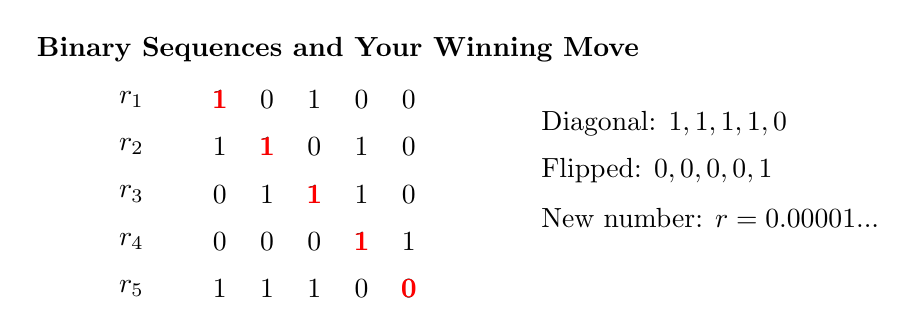
\begin{tikzpicture}[scale=1.2]

    % Table boundaries
    %\draw (0,0) -- (3.5,0);
    %\draw (0,-2.5) -- (3.5,-2.5);
    
    % Table rows
    %\foreach \y in {0,-0.5,-1,-1.5,-2,-2.5} {
    %    \draw (0,\y) -- (3.5,\y);
    %}
    
    % Labels for rows
    \node[left] at (-0.2,0) {\( r_1 \)};
    \node[left] at (-0.2,-0.5) {\( r_2 \)};
    \node[left] at (-0.2,-1) {\( r_3 \)};
    \node[left] at (-0.2,-1.5) {\( r_4 \)};
    \node[left] at (-0.2,-2) {\( r_5 \)};
    
    % Binary values
    \node at (0.5,0) {1};  \node at (1,0) {0};  \node at (1.5,0) {1};  \node at (2,0) {0};  \node at (2.5,0) {0};
    \node at (0.5,-0.5) {1};  \node at (1,-0.5) {1};  \node at (1.5,-0.5) {0};  \node at (2,-0.5) {1};  \node at (2.5,-0.5) {0};
    \node at (0.5,-1) {0};  \node at (1,-1) {1};  \node at (1.5,-1) {1};  \node at (2,-1) {1};  \node at (2.5,-1) {0};
    \node at (0.5,-1.5) {0};  \node at (1,-1.5) {0};  \node at (1.5,-1.5) {0};  \node at (2,-1.5) {1};  \node at (2.5,-1.5) {1};
    \node at (0.5,-2) {1};  \node at (1,-2) {1};  \node at (1.5,-2) {1};  \node at (2,-2) {0};  \node at (2.5,-2) {0};
    
    % Diagonal highlights
    \node[red] at (0.5,0) {\textbf{1}};
    \node[red] at (1,-0.5) {\textbf{1}};
    \node[red] at (1.5,-1) {\textbf{1}};
    \node[red] at (2,-1.5) {\textbf{1}};
    \node[red] at (2.5,-2) {\textbf{0}};
    
    % Right-hand explanation
    \node[right] at (3.8,-0.25) {Diagonal: \( 1,1,1,1,0 \)};
    \node[right] at (3.8,-0.75) {Flipped: \( 0,0,0,0,1 \)};
    \node[right] at (3.8,-1.25) {New number: \( r = 0.00001... \)};
    
    % Title
    \node[above] at (1.75,0.3) {\textbf{Binary Sequences and Your Winning Move}};
    
\end{tikzpicture}
\end{center}

\caption{No matter what list someone gives you, you can always build a number they missed. \textbf{Conclusion:} There’s no way to list all real numbers between 0 and 1. They’re simply too infinite. The real numbers are \textbf{uncountable}.}
\end{figure}










Let’s walk through a specific example of how Cantor’s diagonalization argument works in practice: using binary numbers between 0 and 1. 

\textbf{The goal?} Outsmart someone who claims they’ve listed them all. 

\textbf{Your mission:} construct a binary number that’s guaranteed to be missing from their list.

Now, let’s see how this showdown plays out...

\begin{verbatim}
user1: Alright, I've done it. I've listed *every* binary number 
        between 0 and 1. All of them. Every. Single. One.

user2: Oh? Bold claim. Mind if I test it?

user1: Be my guest. Pick any number — it’s already on the list. Trust me.

*** [cue dramatic zoom] ***
(You, the thoughtful skeptic, lean in. You know exactly how to break this.)

user2: Okay, here’s what I’ll do. I’m going to take the first digit 
        of the first number, the second digit of the second number, 
        the third of the third… you get the idea.

user1: Uh... sure. Knock yourself out.

user2: And now I’m going to flip each of those digits.
        If it’s a 1, I make it 0. If it’s 0, I make it 1.

user1: Wait… what?

user2: I call it the “Diagonal Flip of Doom.” 
        The number I just created is different from every number 
        in your list — at least one digit is off in each row.

user1: -_-

user2: So your list? Not complete. You missed mine.

*** [4th wall commentary] ***
No matter how you try to list all the real numbers between 0 and 1 
in binary, someone can always pull this move — flipping the diagonals 
and creating a number that *can’t* be on the list.

user1: So you're saying... my infinite list... isn't infinite enough?

user2: Exactly. Welcome to uncountability, my friend. :)
\end{verbatim}


\medskip

\noindent
\textbf{Conclusion:} You win the game. There’s no way to list all the real numbers. There are simply \textit{too many of them}. That’s what it means for them to be \textbf{uncountable}.


  

\begin{tcolorbox}[colback=gray!5!white, colframe=black!80!white, title={Historical Sidenote: Nicholas of Cusa and the Paradox of the Infinite}]

  \textbf{Nicholas of Cusa} (1401–1464), a Renaissance cardinal and mystic philosopher, proposed a radical idea for his time: that the infinite is beyond comprehension not because it is vague, but because it is \textit{too precise} — too complete, too whole, too absolute.
  
  In his work \textit{De Docta Ignorantia} (“On Learned Ignorance”), Cusa described God as an **infinite circle whose center is everywhere and circumference nowhere**. He believed that the infinite cannot be approached by finite reasoning — that all human knowledge of it must be paradoxical, asymptotic, and indirect.
  
  \medskip
  
  Though separated by centuries, Cusa’s theology of divine infinity echoed in Cantor’s conviction that the **absolute infinite** could be conceived only as a concept in the mind of God — beyond mathematics, beyond measure, but not beyond meaning.
  
\end{tcolorbox}


\begin{figure}[H]
\centering
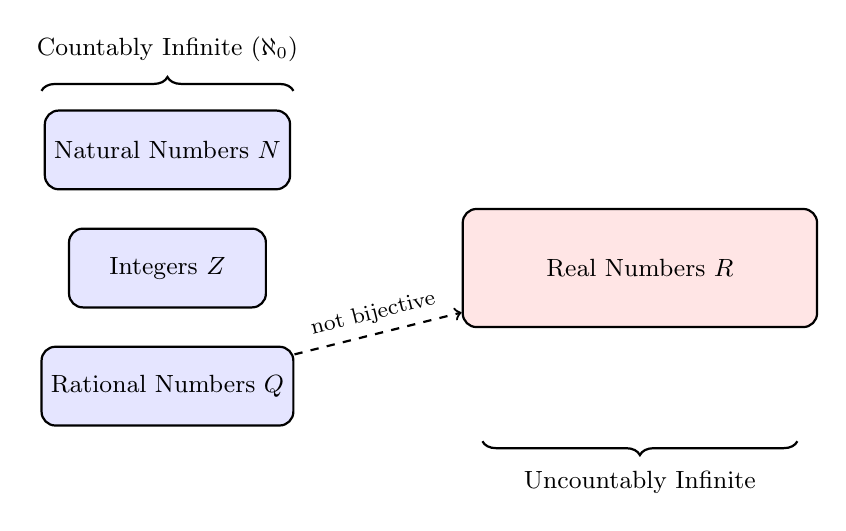
\begin{tikzpicture}[
    every node/.style={font=\small},
    countable/.style={draw, rounded corners=5pt, fill=blue!10, thick, minimum height=1cm, minimum width=2.5cm},
    uncountable/.style={draw, rounded corners=5pt, fill=red!10, thick, minimum height=1.5cm, minimum width=4.5cm}
]

% Countable sets
\node[countable] (naturals) at (0, 0) {Natural Numbers $\mathbb{N}$};
\node[countable] (integers) at (0, -1.5) {Integers $\mathbb{Z}$};
\node[countable] (rationals) at (0, -3) {Rational Numbers $\mathbb{Q}$};

% Uncountable set
\node[uncountable] (reals) at (6, -1.5) {Real Numbers $\mathbb{R}$};

% Top brace for countable sets
\draw[decorate,decoration={brace,amplitude=5pt}, thick]
  (-1.6,0.75) -- (1.6,0.75)
  node[midway,yshift=15pt,align=center] {Countably Infinite ($\aleph_0$)};

% Bottom brace for uncountable sets
\draw[decorate,decoration={brace,mirror,amplitude=5pt}, thick]
  (4,-3.7) -- (8,-3.7)
  node[midway,yshift=-15pt,align=center] {Uncountably Infinite};

% Arrow from Q to R
\draw[->, thick, dashed] (rationals) -- (reals) node[midway, above, sloped] {\footnotesize not bijective};

\end{tikzpicture}
\caption{Cantor's view of infinity: countable sets vs. the uncountable real numbers}
\end{figure}


































\subsection{The Infinite Outsider: Cantor and the Cost of a New Reality}


This led him to introduce the concept of \textbf{infinite cardinalities}, and with it, the now-iconic symbols: the \textbf{aleph numbers}.

\[
\aleph_0\ (\text{aleph-null}) = \text{the cardinality of the natural numbers}
\]

This was the smallest level of infinity: the size of any set you can count, even if it takes forever.

But the real numbers? They’re on another level entirely. A bigger kind of infinite. Cantor didn’t assign a specific aleph to that size—but he knew it was strictly greater than $\aleph_0$.

\[
\text{cardinality of the real numbers} > \aleph_0
\]

Cantor believed the real numbers had cardinality $\aleph_1$—the next step up from $\aleph_0$—a claim known as the \textbf{Continuum Hypothesis}, which remains one of the most famous open questions in mathematics (or rather, one of the most famously undecidable).





\textbf{Infinity, it turned out, came in layers.} And this revelation didn’t win him much praise at the time.





Instead of a Fields Medal, Cantor earned a long list of critics. Many of his contemporaries found the very idea of different infinities absurd—even dangerous. Some accused him of corrupting mathematics with metaphysical nonsense. The stress eventually led to periods of mental illness and professional exile.

But today, we recognize his work as a turning point. Cantor didn’t just discover a new branch of mathematics—he invented the language we now use to talk about the infinite.


\begin{tcolorbox}[colback=gray!5!white, colframe=black!80!white, title={Historical Sidenote: Augustine, Cantor, and the Divine Infinite}]

  \textbf{St. Augustine} (354–430) believed that mathematical truths — number, order, and even infinity — dwell not in the material world, but in the \textit{eternal mind of God}. In works like \textit{Confessions} and \textit{De Libero Arbitrio}, he argued that God’s knowledge is infinite, immediate, and timeless — containing all numbers and all truths at once.

  \medskip

  This idea had a profound afterlife in the work of \textbf{Georg Cantor} (1845–1918), a devout Lutheran who studied theology and saw mathematics as a form of revelation. He viewed the infinite not as a paradox to be tamed, but as a glimpse into the mind of God. In his writings, he referred to the **“absolute infinite”** — not as a mathematical object, but as a symbol of divine perfection, unreachable by reason alone.

  \medskip

  For Cantor, to do mathematics was to participate — however faintly — in the thoughts of God. Set theory wasn’t just rigorous; it was sacred.
  
\end{tcolorbox}





\begin{figure}[H]
\centering
\begin{tikzpicture}[every node/.style={font=\footnotesize}]

% Panel 1: Cantor excited
\comicpanel{0}{4}
  {Cantor}
  {Colleague}
  {\textbf{Cantor:} I’ve discovered a new kind of infinity! Some are bigger than others!}
  {(0,-0.5)}

% Panel 2: Colleague reacts
\comicpanel{6.5}{4}
  {Cantor}
  {Colleague}
  {\textbf{Colleague:} What does that even mean? Infinity is infinity.}
  {(0,-0.5)}

% Panel 3: Cantor explains
\comicpanel{0}{0}
  {Cantor}
  {Colleague}
  {\textbf{Cantor:} You can list the rationals, but not the reals. It's about cardinality!}
  {(0,-0.5)}

% Panel 4: Colleague dismisses
\comicpanel{6.5}{0}
  {Cantor}
  {Colleague}
  {\textbf{Colleague:} That’s not math. That’s metaphysics.}
  {(0,-0.5)}

\end{tikzpicture}
\caption{Cantor tries to introduce a new mathematical reality. His colleagues... weren’t ready.}
\end{figure}







\subsection{The Cantor Set }

To understand why Cantor’s discoveries were so unsettling, let’s look at the \textbf{Cantor set}—one of the first mathematical objects to give analysts an existential crisis.

\begin{itemize}
    \item Start with the interval \( [0,1] \).
    \item Remove the middle third, leaving two intervals: \( [0,1/3] \cup [2/3,1] \).
    \item Remove the middle third from each remaining interval, and repeat indefinitely.
\end{itemize}

Or, more mathematically, What remains is a \textbf{nowhere-dense} set: no intervals, no clusters, just infinitely many points that never add up to anything continuous.

\begin{figure}[H]
\centering
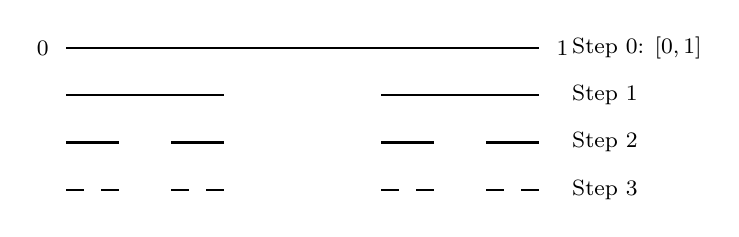
\begin{tikzpicture}[scale=6]

% Level 0: [0,1]
\draw[thick] (0,0) -- (1,0);
\node[anchor=west] at (1.05, 0) {\footnotesize Step 0: $[0,1]$};

% Level 1: remove middle third
\draw[thick] (0, -0.1) -- (1/3, -0.1);
\draw[thick] (2/3, -0.1) -- (1, -0.1);
\node[anchor=west] at (1.05, -0.1) {\footnotesize Step 1};

% Level 2: remove middle third from each remaining interval
\draw[thick] (0, -0.2) -- (1/9, -0.2);
\draw[thick] (2/9, -0.2) -- (1/3, -0.2);
\draw[thick] (2/3, -0.2) -- (7/9, -0.2);
\draw[thick] (8/9, -0.2) -- (1, -0.2);
\node[anchor=west] at (1.05, -0.2) {\footnotesize Step 2};

% Level 3: further removal
\draw[thick] (0, -0.3) -- (1/27, -0.3);
\draw[thick] (2/27, -0.3) -- (1/9, -0.3);
\draw[thick] (2/9, -0.3) -- (7/27, -0.3);
\draw[thick] (8/27, -0.3) -- (1/3, -0.3);

\draw[thick] (2/3, -0.3) -- (19/27, -0.3);
\draw[thick] (20/27, -0.3) -- (7/9, -0.3);
\draw[thick] (8/9, -0.3) -- (25/27, -0.3);
\draw[thick] (26/27, -0.3) -- (1, -0.3);
\node[anchor=west] at (1.05, -0.3) {\footnotesize Step 3};

% Labels
\node at (-0.05, 0) {\footnotesize 0};
\node at (1.05, 0) {\footnotesize 1};

\end{tikzpicture}
\caption{Construction of the Cantor Set: repeatedly removing the middle third}
\end{figure}


In normal language? It’s a set so weird that it contains infinitely many points but takes up no space. It was the first clear example that classical ideas about "size" completely fell apart under set theory.

How do we know it has cardinality as the real numbers? One way to prove it is by recognizing that every point in the Cantor set corresponds to a decimal number made up only of 0s and 2s.

\begin{enumerate}
	\item Each constructed decimal number corresponds to a point in the real interval $[0,1]$.
	\item Since the set of infinite binary sequences has the same cardinality of the reals, so does the Cantor set.
\end{enumerate}

\begin{figure}[H]
\centering
\resizebox{\textwidth}{!}{
\begin{tikzpicture}[node distance=1.0cm and 1cm, >=Latex]

% Ternary representation
\node (ternaryLabel) {\textbf{Ternary (base-3)}: uses only 0s and 2s};
\node[below=of ternaryLabel] (ternary) {\Large $0.202200\ldots_3$};

% Binary representation 
\node[right=1.5cm of ternaryLabel] (binaryLabel) {\textbf{Binary (base-2)}: standard real number encoding};
\node[below=of binaryLabel] (binary) {\Large $0.101100\ldots_2$};

% Real number in Cantor set
\node[below=of ternary, yshift=-1.2cm] (realLine) {\textbf{Point in Cantor set} $\subset [0,1]$};

% Arrows (line length now shorter)
\draw[->, thick] (ternary) -- (binary) node[midway, above, sloped] {\small map 0 $\to$ 0, 2 $\to$ 1};
\draw[->, thick] (binary) -- (realLine);

% Braces or annotation
\node[align=center, below=of realLine, yshift=-0.4cm] (note) {
Each ternary expansion with only 0s and 2s \\ corresponds uniquely to a binary expansion, \\ and thus to a point in $[0,1]$.
};

\end{tikzpicture}
}
\caption{Mapping Cantor set elements (base-3 with 0s and 2s) to binary expansions}
\end{figure}



To get a feel for just how strange the Cantor set really is, imagine you’re chatting with someone who claims to understand it perfectly. Naturally, you're curious — after all, it's supposed to be a set that's both "infinitely full" and yet takes up no space at all. What follows is a conversation where you try to wrap your head around this bizarre construction, and end up questioning whether "size" even makes sense when infinity is involved.


{\ttfamily
\textbf{user1:} Ever heard of the Cantor set?

\textbf{user2:} No, what is it?

\textbf{user1:} It’s a set of numbers between 0 and 1 that contains infinitely many points...

\textbf{user2:} Okay...

\textbf{user1:} ...but has size zero.

\textbf{user2:} Uh, what? That’s nonsense. How can something have infinite points and still be size zero?

\textbf{user1:} Depends on what you mean by “size.”

\textbf{user2:} I mean, if it's got stuff in it, shouldn’t it take up space?

\textbf{user1:} Not necessarily. The Cantor set is built by removing the middle third over and over — forever. What’s left is dust.

\textbf{user2:} But infinite dust?

\textbf{user1:} Exactly. Infinitely many points, but no length. You could never “bump into it” by picking a random number.

\textit{*** [4th wall commentary] ***}

(It turns out our usual idea of “size” doesn’t work here — the Cantor set is a set full of points, but somehow takes up no space at all.)

\textbf{user2:} So it’s tiny?

\textbf{user1:} In one sense, yeah. But in another — get this — it’s actually the same size as the real numbers between 0 and 1.

\textbf{user2:} NOPE. I’m out. That makes zero sense.

\textbf{user1:} Here's the trick: Every number in the Cantor set can be written in base 3 using only 0s and 2s.

\textbf{user2:} Like binary, but skip the 1s?

\textbf{user1:} Exactly. And there are just as many of those infinite strings as there are real numbers.

\textbf{user2:} So it’s... empty but full. Small but huge.

\textbf{user1:} Welcome to set theory. :)
}



\begin{tcolorbox}[colback=gray!5!white, colframe=black!80!white, title={Historical Sidebar: Dedekind and Cantor — Architects of the Infinite Continuum}]

  In the late 19th century, mathematics underwent a foundational shift — one that redefined not just how we compute, but what numbers \textit{are}.
  
  \textbf{Richard Dedekind} (1831–1916) constructed the real numbers using what he called \textbf{cuts} in the rational line — partitioning \( \mathbb{Q} \) into two sets whose separation defined an irrational point. This method made the continuum rigorous: a seamless number line built from logical partitions.
  
  \medskip
  
  \textbf{Georg Cantor} (1845–1918), working around the same time, approached the infinite from the opposite direction. Where Dedekind built the continuum by filling in gaps, Cantor **classified infinities themselves** — showing that the continuum had a distinct, higher cardinality than the countable rationals.
  
  \medskip
  
  The two men were close collaborators and deep admirers of each other’s work. Dedekind even helped Cantor publish his early papers and was one of the first to grasp the philosophical depth of his ideas.
  
  Together, they gave mathematics a modern foundation:
  \begin{itemize}
      \item \textbf{Dedekind} formalized continuity.
      \item \textbf{Cantor} mapped infinity.
  \end{itemize}
  
  \textbf{The real line we measure, integrate over, and build our functions on exists thanks to both.}
  
\end{tcolorbox}



\begin{figure}[H]
\centering
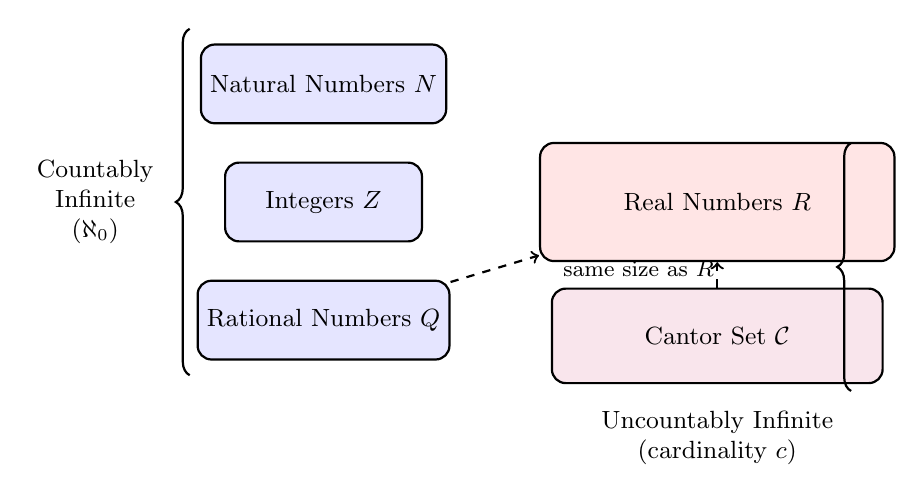
\begin{tikzpicture}[
    every node/.style={font=\small},
    countable/.style={draw, rounded corners=5pt, fill=blue!10, thick, minimum height=1cm, minimum width=2.5cm},
    uncountable/.style={draw, rounded corners=5pt, fill=red!10, thick, minimum height=1.5cm, minimum width=4.5cm},
    special/.style={draw, rounded corners=5pt, fill=purple!10, thick, minimum height=1.2cm, minimum width=4.2cm}
]

% Countable sets
\node[countable] (naturals) at (0, 0) {Natural Numbers $\mathbb{N}$};
\node[countable] (integers) at (0, -1.5) {Integers $\mathbb{Z}$};
\node[countable] (rationals) at (0, -3) {Rational Numbers $\mathbb{Q}$};

% Uncountable sets
\node[uncountable] (reals) at (5, -1.5) {Real Numbers $\mathbb{R}$};
\node[special] (cantor) at (5, -3.2) {Cantor Set $\mathcal{C}$};

% Braces
\draw[decorate,decoration={brace,mirror,amplitude=5pt}, thick]
  (-1.7,0.7) -- (-1.7,-3.7) node[midway,xshift=-1.2cm,align=center] {Countably \\ Infinite \\ ($\aleph_0$)};

\draw[decorate,decoration={brace,mirror,amplitude=5pt}, thick]
  (6.7,-0.75) -- (6.7,-3.9);

% Arrows
\draw[->, thick, dashed] (rationals) -- (reals);
\draw[->, thick, dashed] (cantor) -- (reals);

% Bottom Labels
\node[align=center] at (5, -4.5) {Uncountably Infinite \\ (cardinality $\mathfrak{c}$)};
\node[align=center] at (4, -2.35) {\footnotesize same size as $\mathbb{R}$};

\end{tikzpicture}
\caption{Cantor’s hierarchy: Countable sets vs. uncountable sets like $\mathbb{R}$ and the Cantor set $\mathcal{C}$}
\end{figure}













\subsection{Cantor vs. Kronecker: The Math Feud of the Century}

At this point, you might expect Cantor to have been showered with mathematical awards. Instead, he became the most controversial mathematician in Europe. His biggest enemy? Leopold Kronecker.  

Kronecker, a powerful German mathematician, absolutely despised Cantor’s ideas. He believed that only finite, constructive mathematics was valid and called Cantor a "scientific charlatan." (Yes, that’s an actual quote.)  

But Kronecker wasn’t just throwing insults—he actively sabotaged Cantor’s career:

\begin{itemize}
    \item He blocked Cantor from getting a professorship in Berlin.
    \item He prevented his papers from being published in certain journals.
    \item He used his influence to make Cantor’s work look like academic heresy.
\end{itemize}

And the worst part? It worked. Cantor became increasingly isolated. 


\begin{tcolorbox}[colback=gray!5!white, colframe=black!80!white, title={Historical Sidenote: Constructivism and the Paradox of the Fixed Point}]

  \textbf{Constructivism} is a philosophy of mathematics that insists: to say something exists, you must be able to \textit{construct it}. No appeals to abstract infinities, no non-constructive proofs — only explicit methods, grounded in arithmetic and logic.
  
  This view traces back to \textbf{Kronecker}, and later became central to thinkers like \textbf{Brouwer}, who founded intuitionism in the early 20th century.
  
  \medskip
  
  But many classical theorems defy this approach. One famous example is the \textbf{Brouwer Fixed Point Theorem}, which says:
  
  \begin{quote}
  \textit{Any continuous function from a closed disk to itself has at least one fixed point.}
  \end{quote}
  
  The proof is elegant — but non-constructive. It tells us the fixed point exists, but not how to find it.
  
  \medskip
  
  To a constructivist, this is a problem. Where’s the point? How do you get it? Mathematics, they argue, should not make promises it can’t keep.
  
  Yet the fixed point theorem remains indispensable — in economics, differential equations, game theory, and beyond. Its power lies precisely in its abstract generality — a kind of existence proof that constructivism, on principle, refuses to accept.
  
\end{tcolorbox}


\begin{figure}[H]
\centering
\begin{tikzpicture}[every node/.style={font=\footnotesize}]

% Panel 1: Cantor applying optimistically
\comicpanel{0}{4}
  {Cantor}
  {Kronecker}
  {\textbf{Cantor:} I’ve just applied for the Berlin position. I think my work on infinite sets might finally gain some traction!}
  {(0,-0.5)}

% Panel 2: Kronecker pretending to be polite
\comicpanel{6.5}{4}
  {Cantor}
  {Kronecker}
  {\textbf{Kronecker:} Ah yes, your... imaginative approach to mathematics. How bold of you to redefine reality.}
  {(0,-0.5)}

% Panel 3: Cantor staying firm
\comicpanel{0}{0}
  {Cantor}
  {Kronecker}
  {\textbf{Cantor:} It’s not fantasy—it’s logic. Different infinities follow from clear set-theoretic principles.}
  {(0,0.8)}

% Panel 4: Kronecker dismissing with shade
\comicpanel{6.5}{0}
  {Cantor}
  {Kronecker}
  {\textbf{Kronecker:} Mmm. Well. Perhaps someday philosophy will give you a medal.}
  {(0,0.8)}

\end{tikzpicture}
\caption{Cantor vs. Kronecker: When academic shade became weaponized.}
\end{figure}


\subsection{Cantor’s Later Years: Genius, Madness, and... Shakespeare?}

The constant academic hostility took a toll. Cantor suffered sever mental illness, and was repeatedly institutionalized.

Oh, and did I mention he became obsessed with proving that Shakespeare’s plays were actually written by Francis Bacon? Yes, really. While revolutionizing mathematics, Cantor was also writing academic articles trying to debunk Shakespeare. Very sane. 

Cantor had revolutionized mathematics, but at the cost of his career, his mental health, and, quite possibly, his sanity. His story is a cautionary tale: sometimes, being right doesn’t mean you’ll be accepted. And sometimes, your biggest enemies aren’t your ideas: they’re the gatekeepers who don’t want to hear them.

\begin{figure}[H]
\centering
\begin{tikzpicture}[every node/.style={font=\footnotesize}]

% Panel 1 — Cantor pacing excitedly
\comicpanel{0}{4}
  {Cantor}
  {Colleague}
  {\textbf{Cantor:} I've shown there are infinite sizes of infinity. Also, I’m working on proving Shakespeare was actually Bacon.}
  {(0,-0.5)}

% Panel 2 — Colleague squinting
\comicpanel{6.5}{4}
  {Cantor}
  {Colleague}
  {\textbf{Colleague:} Wait—are you developing transfinite numbers or literary conspiracy theories?}
  {(0,-0.5)}

% Panel 3 — Cantor, completely unbothered
\comicpanel{0}{0}
  {Cantor}
  {Colleague}
  {\textbf{Cantor:} Why not both? Infinity isn’t the only thing that’s uncountable. So are the plot holes.}
  {(0,0.8)}

% Panel 4 — Colleague deadpan
\comicpanel{6.5}{0}
  {Cantor}
  {Colleague}
  {\textbf{Colleague:} This is why they won’t give you the Berlin job.}
  {(0,0.8)}

\end{tikzpicture}
\caption{Cantor's final boss form: transfinite numbers and Shakespearean truth bombs.}
\end{figure}



